% Generated from vacuum_popcorn.md. A plain preprint in the standard article class.
\documentclass[10pt,twocolumn,a4paper]{article}
\usepackage[margin=1.8cm]{geometry}
\usepackage[T1]{fontenc}
\usepackage{mathptmx}
\usepackage{amsmath,graphicx,textcomp}
\usepackage[round,authoryear]{natbib}
\setcitestyle{aysep={}}
\usepackage[hidelinks]{hyperref}
\setlength{\columnsep}{0.6cm}
\title{Vacuum popcorn: ultra-high-energy particles from collapsing false-vacuum pockets}
\author{B. H. Wiseman\\ {\small Independent researcher, Sydney, Australia}\\ {\small benjamin.h.wiseman@gmail.com \quad ORCID 0009-0002-1023-9026}}
\date{Preprint, 2 October 2026}
\begin{document}
\makeatletter
\twocolumn[\begin{@twocolumnfalse}
\maketitle
\begin{abstract}
\noindent First-order phase transitions in the early universe can leave behind pockets of false vacuum that
trap a gas of particles. Inside a pocket the particles are light, and they lack the energy to take
on their larger mass outside it. If such a pocket collapses today (a ``pop''), its wall becomes
ultra-relativistic and throws the trapped particles out, much as fingers pinched together shoot out
a pip. I followed tens of thousands of them through such collapses with exact relativistic
kinematics. A particle that meets the fast-moving wall with energy $E$ leaves with about $m_{\rm
out}^2/4E$, where $m_{\rm out}$ is its mass outside. For a gas at rest and mass ratios up to a
million, the median escapee carries 0.1 to 1.6 per cent of $m_{\rm out}^2/m_{\rm in}$. At larger
ratios most escapees leave with less, but the most energetic tenth still carry 0.05 to 0.5 per cent
of $m_{\rm out}^2/m_{\rm in}$. A particle of $10^7$ GeV outside and 10 GeV inside has a median
escape energy near $10^{20}$ eV, and one of 1 TeV outside and 10 eV inside sends a tenth or more of
its escapees above that. If the escapees decay to photons, Auger's photon limit caps pops in the
Galaxy at about three events a year in a 3000 km\textsuperscript{2} array. The nearest pops would
arrive as several air showers at the same instant from one direction. No experiment has yet searched
for such groups at these energies.
\end{abstract}
\noindent\textbf{Keywords:} Ultra-high-energy cosmic radiation, Cosmic ray sources, Cosmological phase transitions, Particle
astrophysics, Dark matter, Cosmic ray showers
\vspace{1.5em}
\end{@twocolumnfalse}]
\makeatother

\section{Ingredients}

Air-shower arrays have recorded cosmic rays near $10^{20}$ eV since 1962 \citep{Linsley1963}, and
the sources of the most energetic ones are still unknown. Most proposed sources accelerate charged
nuclei in shocks and jets; a few use relics of the early universe, such as collapsing cosmic
textures \citep{Brandenberger2020} or vacuum bubbles seeded by merging black holes
\citep{Sakharov2025}. This letter's recipe needs a pocket of false vacuum, a particle light inside
the pocket and heavy outside it, and something that makes the pocket collapse today. Such a collapse
is what this letter calls a pop.

Recent work supplies the pocket and the particle together. When a first-order phase transition gives
a particle a large mass in the new vacuum, particles without the energy to take on that mass cannot
enter it \citep{Baker2020}. They pile up in the shrinking remnants of the old vacuum. Those remnants
are the Fermi balls of \citet{Kawana2022b} and, where a hot axion gas holds the pocket open, the
axion relic pockets of \citet{Carenza2024}. What makes a pocket collapse today is less settled.
Fermi balls can collapse late, into black holes, possibly as late as today
\citep{Lu2023,Picker2023}. \citet{Khater2026} note that the smallest axion relic pockets, which hold
only a few axions, should classically collapse, and they leave that case for future work.

As far as I can find, no one has worked out what the trapped particles carry away when a pocket
collapses. \citet{Lewicki2023}, who simulated such collapses, found that the particles slow or even
reverse them, and that a pocket can shrink to nothing only if they all escape first. This letter
computes what escapes, with what energy, and how Earth would see it: as air showers that arrive
together (Figure 1).

\begin{figure*}
  \centering
  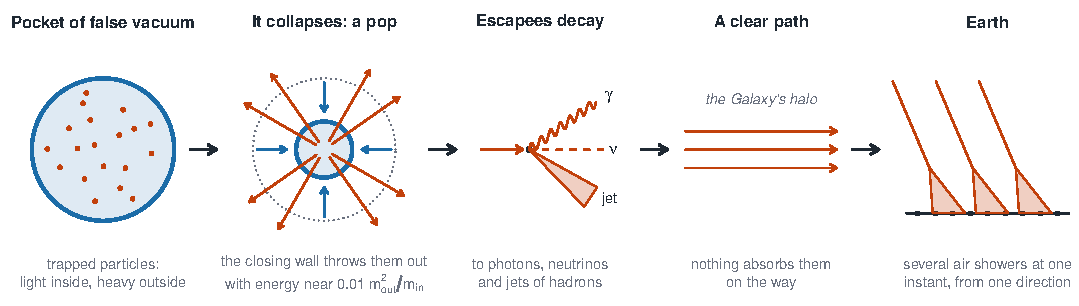
\includegraphics[width=\textwidth]{../fig_schematic.pdf}
  \caption{A pop, from pocket to air showers. A pocket of false vacuum holds particles that are light inside it
    and heavy outside. When it collapses, its wall throws them out. They decay, their products cross the
    Galaxy's halo unabsorbed, and they reach Earth as air showers that arrive together from one
    direction.}
  \label{fig:schematic}
\end{figure*}

\section{Pinching a pip}

Pinch a wet melon pip between finger and thumb and it flies off far faster than your fingers closed.
A collapsing pocket does the same to the particles it traps, and its kinematics can be written down
exactly.

Take a wall moving with Lorentz factor $\gamma$ into a region where a particle has mass $m_{\rm
in}$, with mass $m_{\rm out} > m_{\rm in}$ behind the wall. In the wall's frame energy is conserved,
and the particle crosses only if its momentum normal to the wall, $u$, satisfies $u^2 > m_{\rm
out}^2 - m_{\rm in}^2$. Otherwise the wall reflects it \citep{Dine1992,Arnold1993,Lewicki2023}. A
particle at rest that the wall reflects leaves with energy $\gamma^2(1+\beta^2)\,m_{\rm in} \approx
2\gamma^2 m_{\rm in}$ \citep{Kawana2022a,GarciaGarcia2023}. Any wall conserves the particle's
momentum along it, $p_\perp$. A wall moving at nearly the speed of light also conserves its
light-cone momentum $E + p_n$, where $p_n$ is its momentum along the normal pointing out of the
pocket \citep{Bodeker2009}. Walls this fast have been studied as particle accelerators in the early
universe \citep{Baldes2025,Shakya2024}.

From the conservation of $E + p_n$, a particle at rest that such a wall sweeps up leaves with
\begin{equation}
  E = \frac{m_{\rm out}^2 + m_{\rm in}^2}{2\,m_{\rm in}},
  \label{eq:1}
\end{equation}
and one that meets the wall head-on with energy $E \gg m_{\rm in}$ leaves with
\begin{equation}
  E' = E + \frac{m_{\rm out}^2}{4E}.
  \label{eq:2}
\end{equation}
The less energy a particle brings to the wall, the more it takes away; the wall's motion supplies
the difference. For any reflection, conserving energy in the wall's frame ties the lab energies
before and after it, now written $E$ and $E'$, through $E\,E' = \gamma^2 (m_{\rm in}^2 + p_\perp^2)
+ u^2$, with $u$ again the normal momentum in that frame. A particle reflected from rest therefore
leaves with at most $(2m_{\rm out}^2 - m_{\rm in}^2)/m_{\rm in}$, because a faster wall would let it
through instead.

\section{Following a collapse}

A thin wall in flat space that starts from rest at radius $R_0$ has, by energy conservation, Lorentz
factor
\begin{equation}
  \gamma(x) = \frac{k(1 - x^3) + 1}{x^2}, \qquad x = \frac{R}{R_0}, \qquad k = \frac{\epsilon R_0}{3\sigma},
  \label{eq:3}
\end{equation}
where $\epsilon$ is the vacuum energy released per unit volume and $\sigma$ the wall tension. Small
$k$ means tension drives the collapse, large $k$ means vacuum energy does. Near the centre $\gamma$
grows as $1/R^2$, and a particle that the wall reaches late meets it moving close to the speed of
light.

I followed trapped particles through such collapses one encounter at a time, letting each fly
straight between encounters and applying the exact rule at each. A particle starts from a random
point in the pocket, either at rest or with a thermal or degenerate momentum. One that starts at
rest only ever moves along a radius, and the others I follow in three dimensions. A pocket ends when
it has shrunk to its own wall thickness, a fraction $x_{\rm min}$ of its starting size; particles
still inside then belong to the wall's final burst, which this letter does not follow. Appendix A
describes the numerical method and its checks.

\section{What comes out}

Figure 2 shows the escapees. For a gas at rest with $m_{\rm out}/m_{\rm in}$ between $10^4$ and
$10^6$, the median particle leaves with 0.5 to 1.6 per cent of $m_{\rm out}^2/m_{\rm in}$ when
tension drives the collapse or shares it evenly ($k \le 1$). It leaves with about 0.1 per cent when
vacuum energy drives it ($k = 10$). The spread is one to two decades between the 10th and 90th
percentiles. Between half and nine-tenths of the escapees take the same route. A still-slow wall
hits them once, giving them energy $E_1$. They cross the centre and leave through the far side of
the wall, by then ultra-fast, with between $E_1 + m_{\rm out}^2/4E_1$ and $m_{\rm out}^2/2E_1$,
close to what equation (2) gives. Where each particle sat sets its $E_1$, which is why the spread is
wide. The rest bounce more than once, often after the wall catches them up from behind. When $m_{\rm
out}/m_{\rm in} = 100$, up to 6 per cent of all escapees leave above the reflection limit of section
2, which holds only for head-on bounces.

At larger mass ratios the far side of the wall is often still too slow to let a particle through on
its first return. The particle is thrown back again and gains energy at each extra bounce, and
because equation (2) gives less to a particle that arrives with more, it finally leaves with less
than a single bounce would have given it. The median then falls, by an amount that depends on how
far the pocket shrinks. The most energetic tenth of the escapees still carry 0.2 to 0.5 per cent of
$m_{\rm out}^2/m_{\rm in}$ at a ratio of $10^{10}$ and 0.05 to 0.2 per cent at $10^{12}$. Those
figures are for pockets that end between $10^{-12}$ and $10^{-15}$ of their starting size, the range
that pockets of $10^{15}$ to $10^{20}$ g reach.

In a hot or degenerate gas the particles' typical energy $E_{\rm typ}$ takes the place of $m_{\rm
in}$. The median escapee carries 18 to 23 per cent of $m_{\rm out}^2/E_{\rm typ}$ when $m_{\rm
out}/E_{\rm typ} = 10^2$, and 1.9 to 2.9 per cent when it is $10^4$, for thermal and Fermi gases
alike.

Because the outside mass enters squared, modest masses reach the highest energies. A particle that
weighs $10^7$ GeV outside a pocket and 10 GeV inside it, in a gas at rest with $k \le 1$, has a
median escape energy near $10^{20}$ eV, and about half its escapees exceed it. One of 1 TeV outside
and 10 eV inside sends a tenth to a quarter of its escapees above $10^{20}$ eV. A hot gas with
$m_{\rm out}/E_{\rm typ} = 10^4$ has a median near $10^{20}$ eV when $m_{\rm out} \approx
4\times10^8$ GeV.

\begin{figure*}
  \centering
  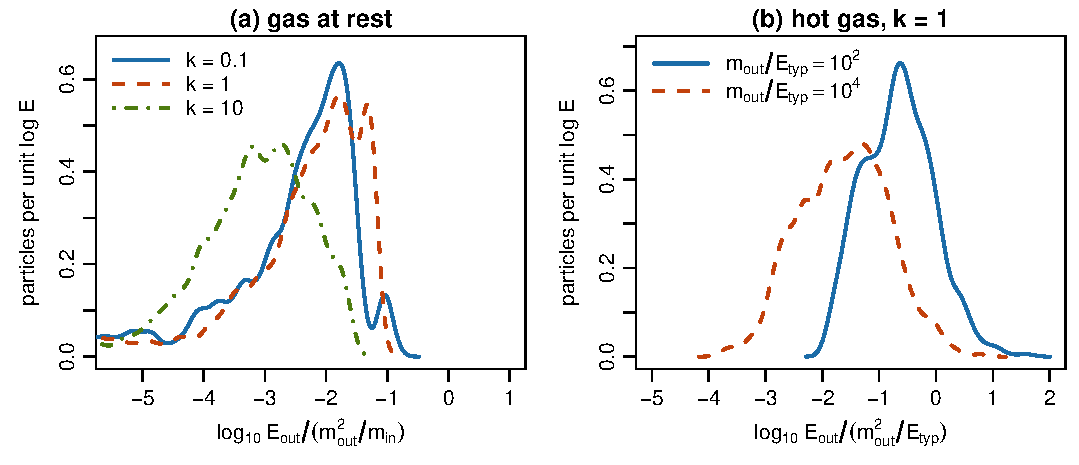
\includegraphics[width=\textwidth]{../fig_spectra.pdf}
  \caption{Energies of the particles that escape a collapsing pocket. (a) A gas initially at rest, $m_{\rm
    out}/m_{\rm in} = 10^6$, in a pocket that ends at $10^{-12}$ of its starting radius, for three wall
    histories. (b) A hot thermal gas, $k = 1$, for two ratios of $m_{\rm out}$ to the gas's typical
    energy.}
  \label{fig:spectra}
\end{figure*}

\section{A pan of popcorn}

What arrives at Earth depends on what the escapees turn into. Outside the pocket their extra mass
opens decay channels that were closed inside, and only their decay products can be seen: photons,
neutrinos and quark jets. The jets make mostly pions, which end as photons and neutrinos, with few
nucleons and no heavier nuclei. Pops therefore cannot supply the bulk of the highest-energy cosmic
rays, which Auger finds to be mostly heavier nuclei \citep{PierreAugerCollaboration2017}.

If the pockets are part of the Galaxy's dark matter, the Galaxy pops like a pan of popcorn, one
pocket at a time, and photons from its pops reach us. Above $10^{18}$ eV their attenuation length
exceeds the size of the halo \citep{Kalashev2016}, and the shortest published interaction length at
$10^{19}$ to $10^{20}$ eV, with the radio background included, is about 1.6 Mpc \citep{Nitu2021}.
Suppose each pop puts a fraction $f$ of its pocket's rest energy into escapees of $10^{20}$ eV that
decay to photon pairs, at a rate $\Gamma$ per pocket. Take a standard halo (\citealp{Navarro1997};
scale radius 20 kpc, 0.4 GeV cm$^{-3}$ at the Sun). Auger's limit on photons above 40 EeV,
$1.72\times10^{-4}$ km$^{-2}$ sr$^{-1}$ yr$^{-1}$ \citep{PierreAugerCollaboration2023a}, then caps
$f\Gamma$ at $1.6\times10^{-32}$ s$^{-1}$, which allows no more than $7\times10^{-15}$ of the
pockets' rest energy to pop in a Hubble time. At that cap a 3000 km\textsuperscript{2} array seeing
the whole sky would record about 3 such events a year, whatever the pocket mass.

A few of the best-known events could have been pops. As a photon, only the 320 EeV Fly's Eye event
of 1991 could \citep{Risse2006}. Telescope Array's 244 EeV event of 2021 was not a photon
\citep{TelescopeArrayCollaboration2023}, and nor were the highest-energy AGASA and Yakutsk events
\citep{Rubtsov2006}. The jets' few nucleons include protons, each with about half to two photons at
the same energy, by the fragmentation ratios of \citet{Aloisio2004}. The searches that found no
photons therefore allow two to ten of Telescope Array's 28 events above 100 EeV to be pop protons,
and ten or more of Auger's 35
\citep{TelescopeArrayCollaboration2026,PierreAugerCollaboration2022,PierreAugerCollaboration2023b}.
The 244 EeV event, whose shower favoured a proton, can be one of them. Telescope Array's ten events
of 2008 to 2013, whose directions are published \citep{TelescopeArrayCollaboration2014}, also lean
toward the Galactic centre, as halo pops would, but Auger's 35 do not.

A pop also arrives all at once. Because its escapees leave within the collapse time and travel at
nearly the speed of light, the decay products of one pop that reach Earth arrive together from one
point. From 1 kpc away they arrive within 5 microseconds of each other if $m_{\rm out} = 1$ TeV, or
within 5 seconds if $m_{\rm out} = 10^6$ GeV. At the photon cap, the share of events that arrive in
simultaneous groups rises with the pocket mass. It is 0.4 per cent for pockets of $10^{15}$ g, 12
per cent for $10^{18}$ g and 70 per cent for $10^{20}$ g, about one group every two years in a 3000
km\textsuperscript{2} array. I found no search by Auger or Telescope Array for simultaneous showers
at these energies; Auger's multiplet searches look for steady sources lined up in arrival direction
and inverse energy \citep{PierreAugerCollaboration2012}. The one search for coincident showers I
know of, CHICOS above $10^{14}$ eV, reported ``a 2.9$\sigma$ excess observed for coincidence times
less than 10 \textmu{}sec'' \citep{Carlson2005}. A particle of 100 GeV outside and 1 MeV inside
would put a pop's showers near $10^{14}$ eV, in the range CHICOS searched, though nothing links that
excess to pops.

\section{What this leaves out}

These results hold until the trapped particles have taken all the pocket's energy. For a gas at rest
that comes when their number times $m_{\rm out}^2/m_{\rm in}$ is 10 to 80 times that energy in five
of the six cases run, and more in the sixth. A heavier load stalls the wall \citep{Lewicki2023}.
Reflection is treated classically, which needs a wall thicker than a particle's wavelength in the
wall's frame. The thrown particle must also be stable inside the pocket and short-lived outside;
that follows if its only Standard Model decays are to heavy states, which are closed inside, where
the particle is light. What makes a relic pocket collapse today is still open.

The rate of pops is free, so no search can exclude them outright, but each claim can fail. An event
shown to be heavier than a proton was not a pop. The 244 EeV event stops being a candidate if
Telescope Array's photon search reaches two to nine times its exposure above $10^{20}$ eV and finds
no photon. And the lean can be tested now. Of Telescope Array's 17 events above 100 EeV with no
published direction \citep{TelescopeArrayCollaboration2023}, an isotropic sky puts one within 50
degrees of the Galactic centre, and the lean of the published ones puts five.

Within those limits, a collapsing pocket throws out the particles it traps, the typical one with a
per cent or less of $m_{\rm out}^2/m_{\rm in}$ and up to 0.2 per cent of them with more than $m_{\rm
out}^2/m_{\rm in}$ itself, and TeV-scale masses can reach $10^{20}$ eV. A nearby pop would reach
Earth as several showers within microseconds to seconds of each other, all from one point. Auger and
Telescope Array record the time of every shower they detect, and their data could be searched for
such groups.

Vacuum decay is usually pictured as the end of the universe, a bubble of lower vacuum that grows at
the speed of light \citep{Coleman1980}. A pop is that physics the other way round. The pocket holds
the higher vacuum, so tension and vacuum energy both push its wall inward, away from us. This kind
of vacuum decay ends the way popcorn does, with a pop, and all that arrives is a handful of air
showers.

\appendix
\section{Numerical method and checks}

At $\gamma = 10^{14}$ a wall moves within five parts in $10^{29}$ of the speed of light, below the
resolution of double-precision arithmetic, and the lag $1/\beta - 1$ cannot be found by subtracting
$\beta$ from 1. The tracker carries that lag, and each particle's light-cone momentum, as quantities
in their own right, and it reduces every timing question to integrals of the lag. Its encounter
formulas agree with 100-digit arithmetic to $5\times10^{-12}$.

For particles at rest the tracker agrees with brute-force time stepping in 36 test collapses, to
$3.3\times10^{-7}$. Leaving out the catch-ups, the encounters in which the wall overtakes a particle
from behind, changes the result in 9 of 18 of those tests. The three-dimensional tracker reproduces
the radial one to $2\times10^{-10}$, and its largest disagreement with brute force,
$1.2\times10^{-3}$, falls to $1.7\times10^{-5}$ when the brute-force time step is cut 25-fold.

\section*{Acknowledgements}

I thank Patricia Karr and all of my wonderful friends and unsuspecting patrons at Kandi Luxe, who
have patiently endured me sounding out ideas on them. And to Winston, you've probably sacrificed at
least one walk to get this paper out, good dog.

I used Claude Opus 5.5 (Anthropic, run in Claude Code, 30 September to 2 October 2026) to write and
check the simulation code, to search the literature and to draft text. Claude Sonnet 5.5 subagents
read the cited sources. MiniMax-M3 and DeepSeek (deepseek-reasoner), through their APIs, proofread
each paragraph in repeated rounds, and I accepted or refused each note. Scripts checked every number
against the code's output and every reference against INSPIRE, and each numerical method was checked
against an independent one, with errors planted to show the check could fail. I reviewed and revised
everything and am responsible for it.

\section*{Financial Support}

This research received no specific grant from any funding agency, commercial, or not-for-profit
sectors.

\section*{Conflicts of Interest}

None.

\section*{Data Availability}

Every number in this letter is produced by a script named for the passage it supports; the code is
at https://github.com/BenWiseman/vacuum-popcorn.

\input{vacuum_popcorn.bbl}

\end{document}
